%%%%%%%%%%%%%%%%%%%%%%%%%%%%%%%%%%%%%%%%%
% Dreuw & Deselaer's Poster
% LaTeX Template
% Version 2.0 (February 18, 2023)
%
% This template originates from:
% https://www.LaTeXTemplates.com
%
% Authors:
% Vel (vel@latextemplates.com)
% Philippe Dreuw and Thomas Deselaers (https://github.com/deselaers/latex-beamerposter)
%
% License:
% CC BY-NC-SA 4.0 (https://creativecommons.org/licenses/by-nc-sa/4.0/)
%
% NOTE: The bibliography needs to be compiled using the bibtex engine.
%
%%%%%%%%%%%%%%%%%%%%%%%%%%%%%%%%%%%%%%%%%

%----------------------------------------------------------------------------------------
%	PACKAGES AND OTHER DOCUMENT CONFIGURATIONS
%----------------------------------------------------------------------------------------

\documentclass{beamer} % Use the beamer base class

\usepackage[
	orientation=portrait, % Portrait orientation
	size=a1, % Paper size
	scale=1.19, % Scale, it's important to adjust this so your content fits nicely in the template
]{beamerposter} % Use the beamerposter package to create the layout

\usetheme{I6pd2} % Use the I6pd2 theme supplied with this template

\usepackage{changepage} % Required for temporarily indenting text blocks

\usepackage{amsmath,amsthm,amssymb,latexsym} % For including math equations, theorems, symbols, etc

\usepackage{gfsdidot} % Use the GFS Didot font

\usepackage{booktabs} % Top and bottom rules for tables

\graphicspath{{Figures/}} % Location of figure images

%----------------------------------------------------------------------------------------
%	TITLE SECTION
%----------------------------------------------------------------------------------------

\title{\LARGE Machin vs. Machine: \\ How Do Neural Networks React to the Unexpected?} % Poster title

\author{\Large By Amelie Machin} % Author(s)

%----------------------------------------------------------------------------------------
%	REMOVE FOOTER
%----------------------------------------------------------------------------------------

\setbeamertemplate{footline}{} % Uncomment this line to hide the footer

%----------------------------------------------------------------------------------------

\begin{document}

\begin{frame}[t] % The whole poster is enclosed in one beamer frame, the [t] parameter aligns everything to the top

\begin{columns}[t] % Begin multi-column layout, the [t] parameter aligns each column's content to the top

\begin{column}{0.02\textwidth}\end{column} % Empty column for horizontal whitespace

%----------------------------------------------------------------------------------------
%	Introductions
%----------------------------------------------------------------------------------------

\begin{column}{0.3\textwidth}%Keyword column

\begin{block}{Introduction}
	\begin{column}{0.75\linewidth}
	The human brain is an incredibly complicated example of biological machinery. It can store information and apply it to a variety of situations to efficiently solve problems, complete tasks, understand the world around them, and adapt to change. This allows humans to not only learn from a guide, but from their own mistakes and past experiences. Neural networks are a subcategory of AI that attempts to recreate this behaviour using code, calculus and matrices. 
	
	\bigskip
	Programs are great at following instructions to get from an expected input to an expected output. However, in the real world, not every piece of data can be anticipated. This research aims to find the similarities and difference between how humans, neural networks, and Large Language Models (such as ChatGPT) react to unexpected inputs through an image classification task with limited class options.
	\bigskip

	\end{column}
	\begin{column}{0.25\linewidth}
		\begin{figure}
		\centering
		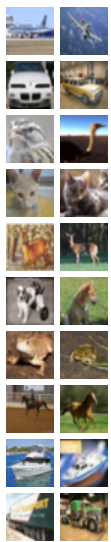
\includegraphics[width=1\textwidth]{CIFARclasses.png}
		\caption{Example images for each class \cite{CIFARImages}}
		\label{fig:CIFARclasses}
		\end{figure}
	\end{column}
	\bigskip

	The limited classes are the 10 classes from the CIFAR-10 dataset: Airplane; Automobile; Bird; Cat; Deer; Dog; Frog; Horse; Ship; Truck. Example images for each class can be seen in figure \ref{fig:CIFARclasses}. 

	\bigskip
	The "unexpected inputs" are 9 images that either have no relation to any of those 10 categories, or images fit a category, but have been heavily distorted. There is also one validation image that does fit a category. All tests were performed with the same 10 images. One example of an image used is below.
	\bigskip

	\begin{figure}
		\centering
		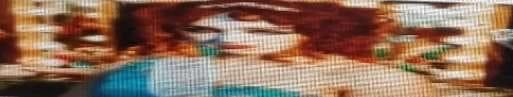
\includegraphics[width=0.9\textwidth]{Chappell.jpg}
		\caption{A stretched image of the singer Chappell Roan.}
		\label{fig:Chappell}
	\end{figure}
\end{block}

\begin{block}{Neural Networks}
	A neural network is an algorithm which mimics the structure of the brain in order to learn, find, or predict patterns in data.

	\begin{figure}[ht]
		\centering
		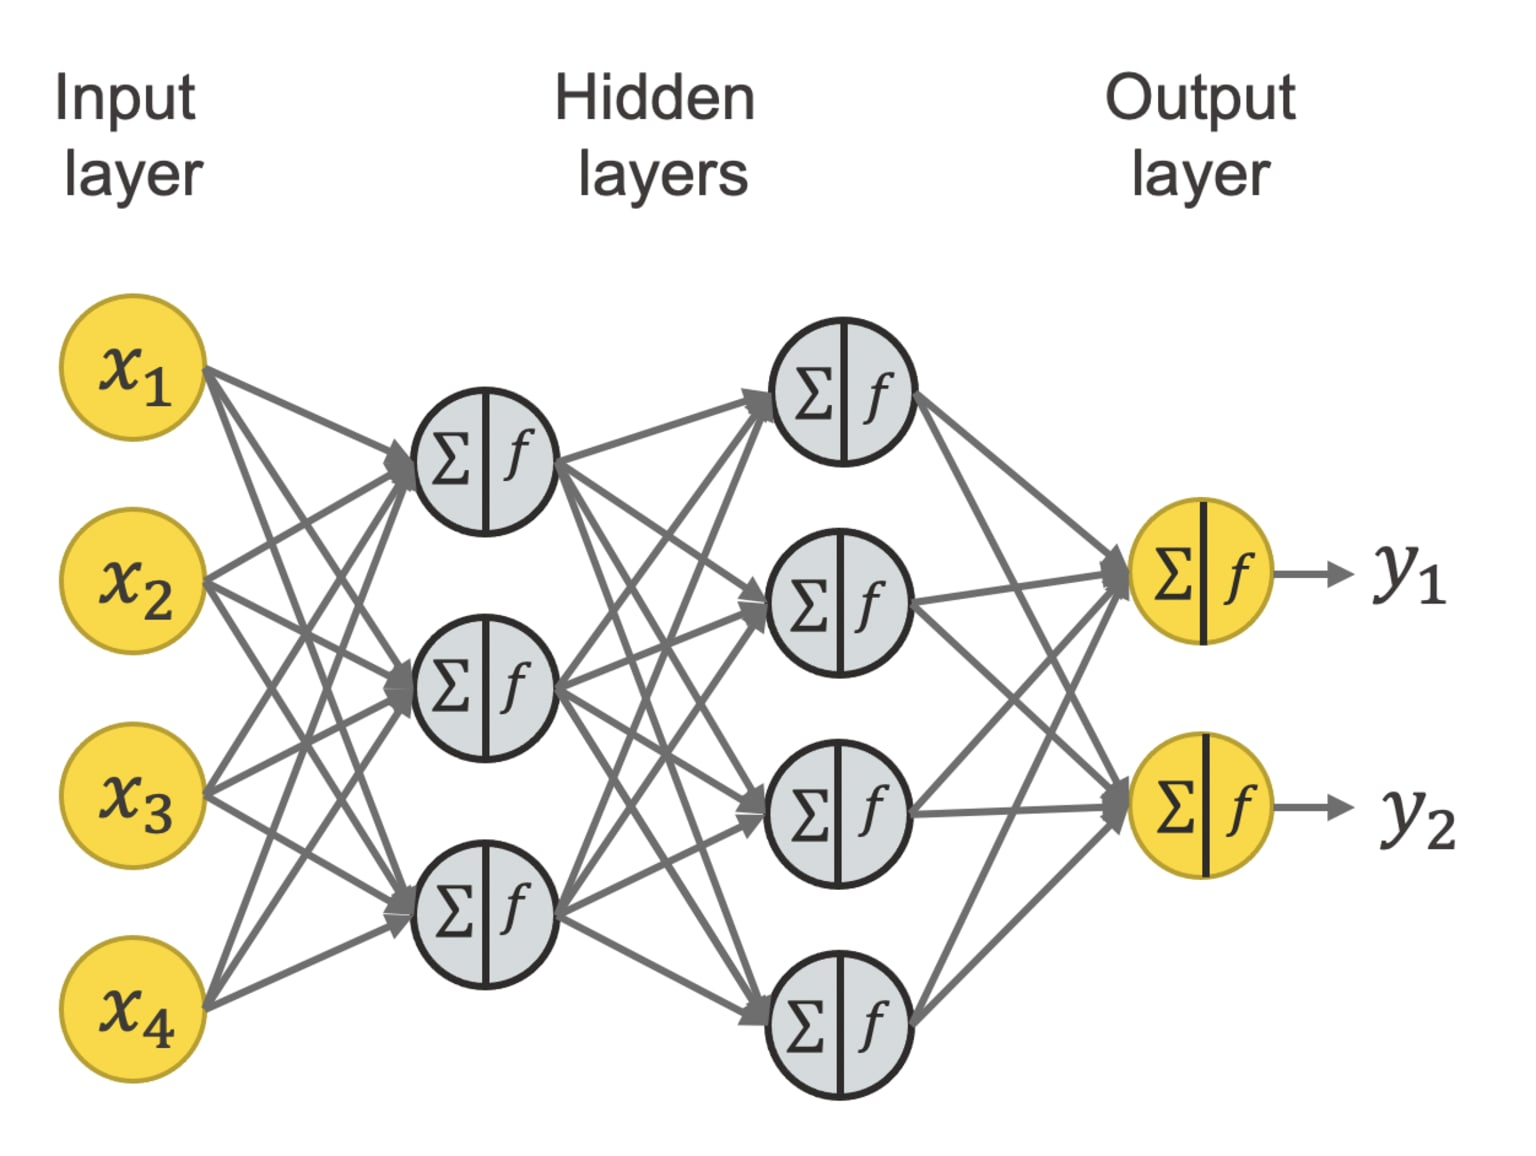
\includegraphics[width=0.96\linewidth]{Figures/neuralNet.jpg}
		\caption{A diagram of a neural network with four layers of nodes. $\Sigma$ represents a linear function and $f$ represents a non-linear activation function. Taken from \cite{knime}}
		\label{fig:netimage}
	\end{figure}

	They are comprised of layers of neurons, called nodes, which perform mathematical functions on the data. Each node has a weight, which represents how much this node affects the output of the network. The network automatically changes these weights while learning patterns in order to make its predictions more accurate.

	\bigskip
	One of the mathematical functions the nodes perform is an activation function, which allows neural networks to learn non-linear (complex) patterns in the data.
\end{block}

\end{column}
%----------------------------------------------------------------------------------------

\begin{column}{0.03\textwidth}\end{column}

\begin{column}{0.3\textwidth} % Start the second content column
            


%----------------------------------------------------------------------------------------
%	MATERIALS
%----------------------------------------------------------------------------------------

\begin{block}{Creating My Own Neural Network}
	I programmed a neural network in Python that takes an image as an input, detects features of the image, and outputs which of CIFAR-10's 10 classes it believes the image best belongs to. It also outputs a confidence score.

	\bigskip
	The neural network was trained on the images and corresponding class labels in CIFAR-10's dataset \cite{krizhevsky2009learning}. The network learned the patterns between the images and the labels it was given, reaching an accuracy of 74\%. Given how small the CIFAR-10 dataset is, and that I had limited resources to train the network, this accuracy is reasonable.
		\begin{figure}[ht]
			\centering
			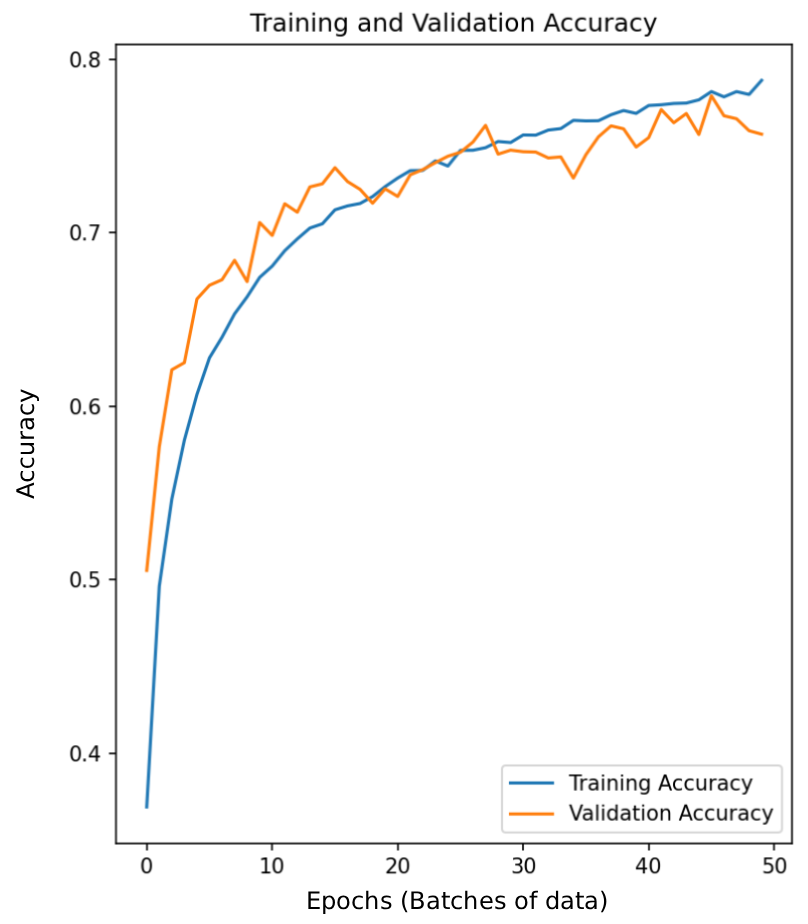
\includegraphics[width=0.696\textwidth]{myNNAcc.png}
			\caption{Graph showing epochs (batches of training data inputted) by accuracy. Blue represents the accuracy of the network on data it was trained on, yellow represents the accuracy of the network on data it was not. The yellow line ends at 0.74, so the network had an accuracy of 74\%.}
			\label{fig:myNNAcc}
		\end{figure}
	
	
\end{block}

%----------------------------------------------------------------------------------------
%	METHODS
%----------------------------------------------------------------------------------------

\begin{block}{Re-training Public Neural Networks}	
	Public neural networks are networks that have been trained by other people using extremely large datasets. This means most of the work towards increasing the accuracy of the network has already been done to a high standard. However, most public image classification neural networks are trained to classify into thousands of categories, so I had to re-train them to only classify into the 10. 
	
	\bigskip
	This process allowed me to get to accuracies of over 90\%.
\end{block}

%----------------------------------------------------------------------------------------
%	MATHEMATICS
%----------------------------------------------------------------------------------------

\begin{block}{Large Language Models}
	Large Language Models are usually the first thing that comes to mind when "AI" is mentioned. They can take inputs in plain English, apply a variety of functions to data both received from the input and gathered from elsewhere, and output in plain English. The LLMs used in this study also have the additional feature of image classification.

	\bigskip
	In the name of science, I provided 4 LLMs -- OpenAI's ChatGPT, Google's Gemini, Microsoft's Copilot, and Claude -- with the 10 images and the same prompt telling it to respond to each image with its chosen class, reasons behind that response, and a confidence score.

	\bigskip
	The prompt forced the LLM to zero-shot its response, which means it had to create its own method for classifying the images. This is in contrast to it relying on instructions, examples or previous training.
\end{block}

\begin{block}{Survey}
	I surveyed 71 people, with 69 of them answering the validation image correctly.

	\bigskip
	Each question featured one of the 10 images, and required one of the 10 categories, a reason, and a score out of 10 as a response.
\end{block}

%----------------------------------------------------------------------------------------

\end{column} % End of the first column

\begin{column}{0.03\textwidth}\end{column} % Empty column for horizontal whitespace
 
\begin{column}{0.3\textwidth} % Start the second content column

%----------------------------------------------------------------------------------------
%	RESULTS
%----------------------------------------------------------------------------------------

%------------------------------------------------

\begin{block}{Results}
	\begin{figure}[ht]
		\centering
		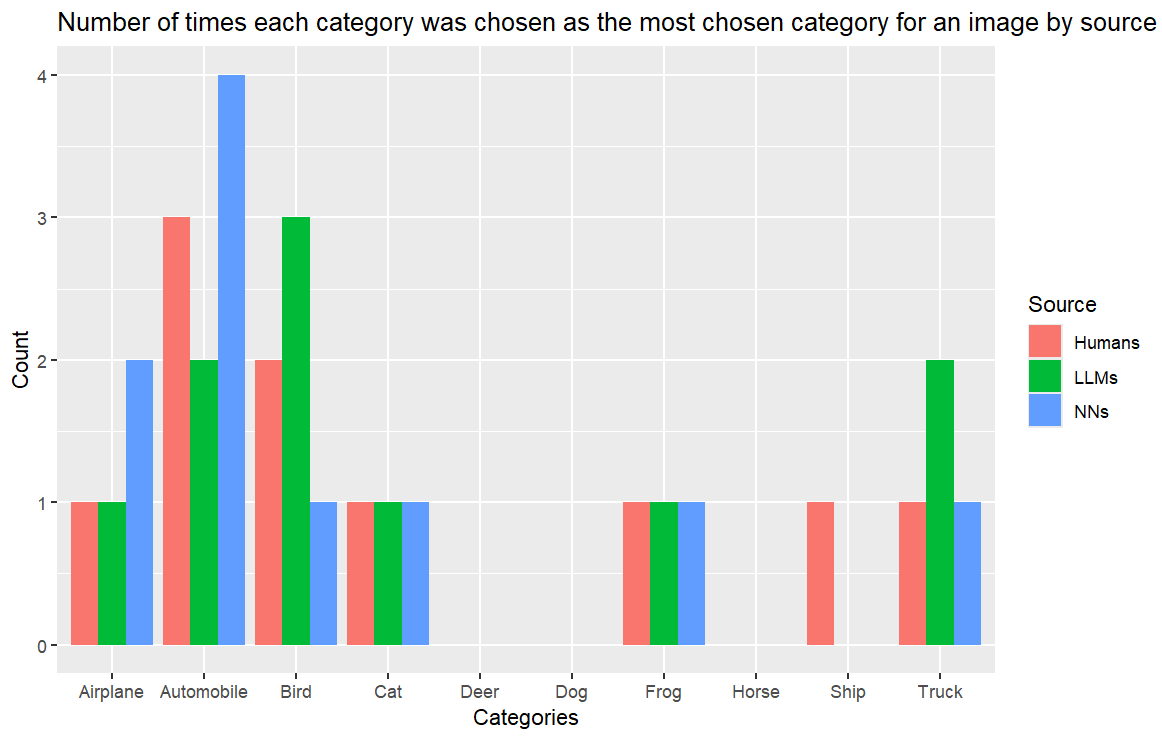
\includegraphics[width=1\linewidth]{CatCount.png}
		\caption{Grouped bar chart showing the number of times each source (humans, LLMs, and neural networks) chose each category as a majority for each of the 10 images.}
		\label{fig:CatCount}
	\end{figure}
	\begin{itemize}
	\item Humans were the most spread out across the categories of the sources. 
	\begin{itemize}
		\item I believe this is because the thought processes that led to classifications varied significantly in creativity between people, leading to a wide range of responses.
		\item This shows that when faced with unexpected data, people are able to make creative leaps in their thought processes to reach a "good enough" response.
	\end{itemize}
	\item The neural networks tended towards the inanimate categories -- such as airplane or automobile -- more than the other sources. 
	\begin{itemize}
		\item I believe this is because neural networks base its response purely off of visual features of the image, and cars and planes have very varied shapes and colours.
		\item This shows that neural networks have little to no versatility, so are somewhat ineffective at handling unexpected data.
	\end{itemize}
	\item The LLMs are quite spread out across the categories. 
	\begin{itemize}
		\item I believe this is because in the reasons they gave, they often mentioned that their choice was arbitrary.
		\item This shows that the LLMs were able to figure out that pure feature extraction was not good enough for classifying images, but were not always able to perform creative leaps, like the humans did, to justify choosing a category.
		\item Some models were better than others at coming up with creative solutions and avoiding arbitrary responses. This shows that LLMs have the capability to improve this result.
	\end{itemize}
	\end{itemize}
\end{block}

%----------------------------------------------------------------------------------------
%	CONCLUSIONS
%----------------------------------------------------------------------------------------

\begin{block}{Conclusions}
	Neural networks react poorly to the unexpected. They assume all data follows their expected inputs, leading to ineffective functions being performed on the data and results far from what a human would expect.

	\bigskip
	On the other hand, Large Language Models show promise at being able to react to the unexpected. Some models were able to perform somewhat creative techniques to find solutions, but are currently far from achieving true creativity and flexibility.

	\bigskip
	Only humans currently have the creativity and flexibility to handle the unexpected situations the real world throws at us. Technology is still stuck in an idealistic world with expected situations.
\end{block}

%----------------------------------------------------------------------------------------
%	REFERENCES
%----------------------------------------------------------------------------------------

\begin{block}{References}
	\nocite{*} % Insert publications even if they are not cited in the poster
	\small % Reduce font size
	\vspace{-1ex} % Pull up slightly
	\bibliographystyle{unsrt} % Bibliography style
	\bibliography{ref.bib} % Bibliography file
\end{block}

%----------------------------------------------------------------------------------------

\end{column} % End of the second column

\begin{column}{0.02\textwidth}\end{column} % Empty column for horizontal whitespace

\end{columns} % End of all the columns in the poster

\end{frame} % End of the enclosing frame

%----------------------------------------------------------------------------------------

\end{document}
